\documentclass[11pt,oneside,openany,headings=optiontotoc,11pt,numbers=noenddot]{article}

\usepackage[a4paper]{geometry}
\usepackage[utf8]{inputenc}
\usepackage[T1]{fontenc}
\usepackage{lmodern}
\usepackage[ngerman]{babel}
\usepackage{ngerman}

\usepackage[onehalfspacing]{setspace}

\usepackage{fancyhdr}
\usepackage{fancybox}

\usepackage{rotating}
\usepackage{varwidth}

%Struktogramme
\usepackage[german,curves]{struktex}

\usepackage{pdflscape}
\usepackage{changepage}
\usepackage{graphicx}
\usepackage[bottom]{footmisc}
\usepackage{transparent}
\usepackage{graphbox}
\graphicspath{
	{Pics/PDFs/}
	{Pics/JPGs/}
	{Pics/PNGs/}
}
\usepackage{caption}
\usepackage{wrapfig}
\usepackage{marginnote}
\usepackage{tabularx}
\usepackage{dashrule}
\usepackage{soulutf8}
\usepackage{hhline}
%arydshln suppresses vertical lines in table
%\usepackage{arydshln}
\usepackage{multirow}
\usepackage{enumerate}
\usepackage[hidelinks]{hyperref}
\usepackage{listings}

\usepackage[table]{xcolor}
\usepackage{array}
\usepackage{enumitem,amssymb,amsmath}
\usepackage{interval}
\usepackage{cancel}
\usepackage{stmaryrd}
\usepackage{wasysym}
\usepackage{polynom}
\usepackage{diagbox}
\usepackage{dashrule}
\usepackage{framed}
\usepackage{mdframed}
\usepackage{karnaugh-map}
\usepackage{pdfpages}

\usepackage{blindtext}

\usepackage{eso-pic}

\usepackage{amssymb}
\usepackage{eurosym}

\usepackage[pages=some]{background}
\pagestyle{headings}
\renewcommand{\headrulewidth}{0.2pt}
\renewcommand{\footrulewidth}{0.2pt}
\newcommand*{\underdownarrow}[2]{\ensuremath{\underset{\overset{\Big\downarrow}{#2}}{#1}}}
\setlength{\fboxsep}{5pt}
\newcommand{\explainBelow}[3]{\underbrace{#1}_{\parbox{\widthof{#3}}{\footnotesize\raggedright #2}}}
\newcommand{\explainAbove}[3]{\overbrace{#1}^{\parbox{\widthof{#3}}{\footnotesize\raggedright #2}}}
\newcommand\footnoteref[1]{\protected@xdef\@thefnmark{\ref{#1}}\@footnotemark}


% Codestyle defined
\definecolor{codegreen}{rgb}{0,0.6,0}
\definecolor{codegray}{rgb}{0.5,0.5,0.5}
\definecolor{codepurple}{rgb}{0.58,0,0.82}
\definecolor{backcolour}{rgb}{0.95,0.95,0.92}
\definecolor{deepgreen}{rgb}{0,0.5,0}
\definecolor{darkblue}{rgb}{0,0,0.65}
\definecolor{mauve}{rgb}{0.40, 0.19,0.28}
\colorlet{exceptioncolour}{yellow!50!red}
\colorlet{commandcolour}{blue!60!black}
\colorlet{numpycolour}{blue!60!green}
\colorlet{specmethodcolour}{violet}

%Neue Spaltendefinition
\newcolumntype{L}[1]{>{\raggedright\let\newline\\\arraybackslash\hspace{0pt}}m{#1}}
\newcolumntype{M}{>{\centering\arraybackslash}X}
\newcommand{\cmnt}[1]{\ignorespaces}
%Textausrichtung ändern
\newcommand\tabrotate[1]{\rotatebox{90}{\raggedright#1\hspace{\tabcolsep}}}

%Intervall-Konfig
\intervalconfig {
	soft open fences
}

%Bash
\lstdefinestyle{BashInputStyle}{
	language=bash,
	basicstyle=\small\sffamily,
	backgroundcolor=\color{backcolour},
	columns=fullflexible,
	backgroundcolor=\color{backcolour},
	breaklines=true,
}
%Java
\lstdefinestyle{JavaInputStyle}{
	language=Java,
	backgroundcolor=\color{backcolour},
	aboveskip=1mm,
	belowskip=1mm,
	showstringspaces=false,
	columns=flexible,
	basicstyle={\footnotesize\ttfamily},
	numberstyle={\tiny},
	numbers=none,
	keywordstyle=\color{purple},,
	commentstyle=\color{deepgreen},
	stringstyle=\color{blue},
	emph={out},
	emphstyle=\color{darkblue},
	emph={[2]rand},
	emphstyle=[2]\color{specmethodcolour},
	breaklines=true,
	breakatwhitespace=true,
	tabsize=2,
}
%Python
\lstdefinestyle{PythonInputStyle}{
	language=Python,
	alsoletter={1234567890},
	aboveskip=1ex,
	basicstyle=\footnotesize,
	breaklines=true,
	breakatwhitespace= true,
	backgroundcolor=\color{backcolour},
	commentstyle=\color{red},
	otherkeywords={\ , \}, \{, \&,\|},
	emph={and,break,class,continue,def,yield,del,elif,else,%
		except,exec,finally,for,from,global,if,import,in,%
		lambda,not,or,pass,print,raise,return,try,while,assert},
	emphstyle=\color{exceptioncolour},
	emph={[2]True,False,None,min},
	emphstyle=[2]\color{specmethodcolour},
	emph={[3]object,type,isinstance,copy,deepcopy,zip,enumerate,reversed,list,len,dict,tuple,xrange,append,execfile,real,imag,reduce,str,repr},
	emphstyle=[3]\color{commandcolour},
	emph={[4]ode, fsolve, sqrt, exp, sin, cos, arccos, pi,  array, norm, solve, dot, arange, , isscalar, max, sum, flatten, shape, reshape, find, any, all, abs, plot, linspace, legend, quad, polyval,polyfit, hstack, concatenate,vstack,column_stack,empty,zeros,ones,rand,vander,grid,pcolor,eig,eigs,eigvals,svd,qr,tan,det,logspace,roll,mean,cumsum,cumprod,diff,vectorize,lstsq,cla,eye,xlabel,ylabel,squeeze},
	emphstyle=[4]\color{numpycolour},
	emph={[5]__init__,__add__,__mul__,__div__,__sub__,__call__,__getitem__,__setitem__,__eq__,__ne__,__nonzero__,__rmul__,__radd__,__repr__,__str__,__get__,__truediv__,__pow__,__name__,__future__,__all__},
	emphstyle=[5]\color{specmethodcolour},
	emph={[6]assert,range,yield},
	emphstyle=[6]\color{specmethodcolour}\bfseries,
	emph={[7]Exception,NameError,IndexError,SyntaxError,TypeError,ValueError,OverflowError,ZeroDivisionError,KeyboardInterrupt},
	emphstyle=[7]\color{specmethodcolour}\bfseries,
	emph={[8]taster,send,sendMail,capture,check,noMsg,go,move,switch,humTem,ventilate,buzz},
	emphstyle=[8]\color{blue},
	keywordstyle=\color{blue}\bfseries,
	rulecolor=\color{black!40},
	showstringspaces=false,
	stringstyle=\color{deepgreen}
}

\lstset{literate=%
	{Ö}{{\"O}}1
	{Ä}{{\"A}}1
	{Ü}{{\"U}}1
	{ß}{{\ss}}1
	{ü}{{\"u}}1
	{ä}{{\"a}}1
	{ö}{{\"o}}1
}

% Neue Klassenarbeits-Umgebung
\newenvironment{worksheet}[3]
% Begin-Bereich
{
	\newpage
	\sffamily
	\setcounter{page}{1}
	\ClearShipoutPicture
	\AddToShipoutPicture{
		\put(55,761){{
				\mbox{\parbox{385\unitlength}{\tiny \color{codegray}BBS I Mainz, #1 \newline #2
						\newline #3
					}
				}
			}
		}
		\put(455,761){{
				\mbox{\hspace{0.3cm}
\includegraphics[width=0.2\textwidth]{../../logo.pdf}}
			}
		}
	}
}
% End-Bereich
{
	\clearpage
	\ClearShipoutPicture
}

\setlength{\columnsep}{3em}
\setlength{\columnseprule}{0.5pt}

\geometry{left=1.50cm,right=1.00cm,top=3.00cm,bottom=1.00cm,includeheadfoot}
\pagestyle{plain}
\pagenumbering{arabic}

\begin{document}
	\begin{worksheet}{Berufliches Gymnasium}{Klassenstufe 12 - Informationsverarbeitung - Leistungskurs}{Lernabschnitt: \textbf{Datenbanken}}
		\setlength{\columnseprule}{0pt}
		
		\section{Datenbanken}
		Dieses Kapitel wird sich mit dem Thema \textbf{Datenbanken} beschäftigen. Bevor wir uns aber mit der Materie auseinandersetzen ein paar interessante Fakten:
		\paragraph{Definition aus dem \glqq{}Duden Informatik\grqq{}} System zur Beschreibung, Speicherung und Wiedergewinnung von umfangreichen Datenmengen, die von mehreren Anwendungsprogrammen genutzt werden. \textit{ff.}
		\subsubsection*{Historie der Datenspeicherung}
		\storestyleof{itemize}
		\begin{listliketab}
			\begin{tabular}{Llll}
				\textbullet & 50er Jahre & Dateisysteme auf Band\\
				\textbullet & 60er Jahre & Dateisysteme auf Platte\\
				& & Dateiverwaltungssysteme (z.B. ISAM)\\
				\textbullet & 70er Jahre & Erste Datenbanksysteme (DBMS)\\
				& & - \hspace{0.2cm} hierarchisches DB-Modell\\
				& & - \hspace{0.2cm} Netzwerkmodell\\
				\textbullet & 80er Jahre & Relationate DBS (RDBS)\\
				\textbullet & 90er Jahre & Postrelationale DBS\\
				& & - \hspace{0.2cm} Objekt-Relationale Systeme (ORDBS)\\
				& & - \hspace{0.2cm} Objektorientiere DBS (OODBS)\\
			\end{tabular}
		\end{listliketab}
		\subsubsection*{Ziel der Entwicklung von DBMS}
		Bis dato gab es zwei Arten der Datenspeicherung: Dateisysteme und Dateiverwaltungssysteme.\\
		\par\noindent
		\begin{minipage}{0.48\textwidth}
			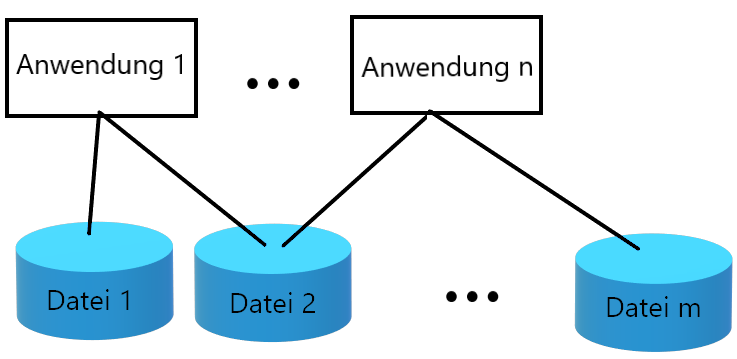
\includegraphics[width=0.98\textwidth]{../99_Bilder/01_Dateisysteme.png}\\
			\texttt{\footnotesize{Abb. 1: Dateisysteme}}
		\end{minipage}
		\hfill
		\begin{minipage}{0.48\textwidth}
			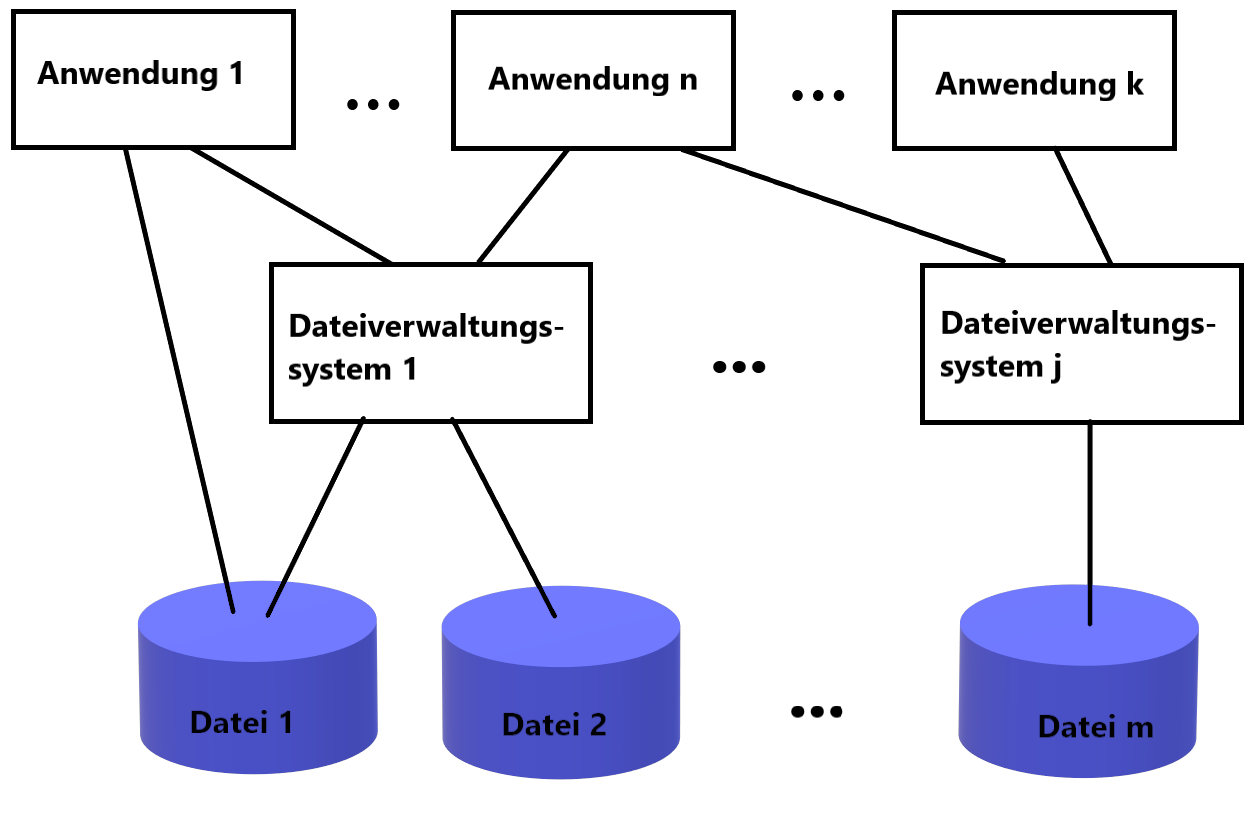
\includegraphics[width=0.98\textwidth]{../99_Bilder/01_Dateiverwaltungssysteme.png}\\
			\texttt{\footnotesize{Abb. 1: Dateiverwaltungssysteme}}
		\end{minipage}
		\newpage
		Probleme beim Einsatz von Dateisysteme:
		\begin{itemize}[label=-]
			\item \textbf{Datenredundanz}\\
			Die gleichen Daten werden von mehreren verschiedenen Dateien gespeichert, z.B. Adressen von Kunden werden von mehreren Anwendungen wie Auftragsabwicklung, Buchhaltung usw. verwaltet.\\
			\textit{Problem:} Speicherplatzverschwendung, Inkonsistenzen
			\item \textbf{Schlechte Effizienz}
			\item \textbf{Problem bei Mehrbenutzerbetrieb}
			\item \textbf{Keine Datenunabhängigkeit}\\
			Anwendungsprogrammierer und Anwender müssen die interne Darstellung der Daten und ihre Organisation (Speicherort etc.) kennen.
			\item Zugriffskontrolle und Datensicherheit sind problematisch
		\end{itemize}
		Bei der Entwicklung von Datenbank-Management-Systemen (DBMS) spielte die \textbf{Datenintegration} eine große Rolle. Das bedeutet:
		\begin{itemize}[label=-]
			\item Alle System- und Anwendungsprogramme arbeiten auf denselben Daten, die von einer \underline{zentralen} Datenkomponente (\grqq{}Datenbank\grqq{}) verwaltet werden.
			\item Dadurch kann nicht nur das Problem der Datenredundanz beseitigt werden, sondern auch andere Probleme können gelöst werden
			\begin{itemize}
				\item Zugriff auf die Daten ohne Kenntnis der konkreten internen Darstellen über standardisierte Zugriffsmechanismen (z.B. Abfragesprachen)
				\item \glqq{}Geordneter\grqq{} Mehrbenutzerbetrieb (Transaktionskonzept)
				\item Zugriffskontrolle und Datensicherheit (z.B. durch zentrale Datensicherungsmechanismen)
				\item Gesteigerte Effizienz durch interne Optimierungsmöglichkeiten des DBMS
			\end{itemize}
			\begin{center}
				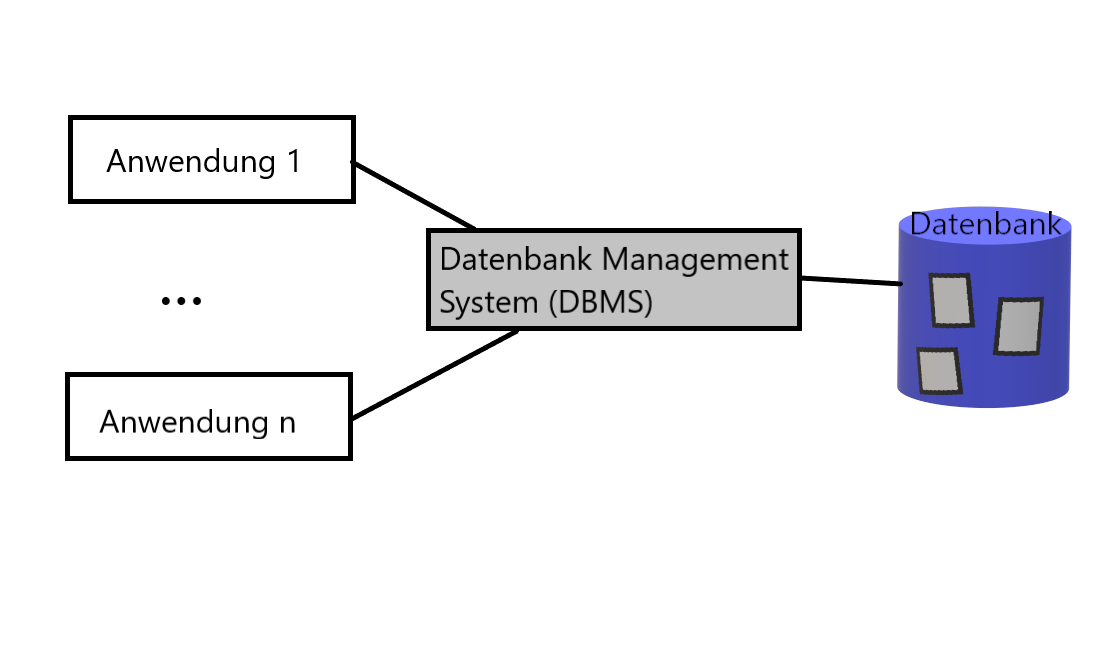
\includegraphics[width=0.75\textwidth]{../99_Bilder/DBMS.png}
			\end{center}
		\end{itemize}
		\section*{Anforderungen an ein DBMS}
		Für einen zuverlässigen und effizienten Einsatz von DBMS hat \textit{Edgar F. Codd} \underline{neun Anforderungen} definiert:
		\begin{itemize}[label=$\circ$]
			\item \textbf{Integration} einheitliche, nicht-redundante Verwaltung aller Anwendungsdaten
			\item \textbf{Operationen} Operationen wie Speicher, Ändern, Löschen und Suchen auf den Daten müssen möglich sein
			\item \textbf{Katalog} dieser ermöglicht Zugriffe auf die Datenbeschreibung (\textit{Data Dictionary})
			\item \textbf{Benutzersichten} Für unterschiedliche Anwendungen werden unterschiedliche Sichten auf den Datenbestand ermöglicht
			\item \textbf{Konsistenzüberwachung} Integritätssicherung: Gewährleistung der Korrektheit des Datenbestandes und der korrekten Ausführung von Änderungen
			\item \textbf{Zugriffskontrolle} Ausschluss von unautorisierten Zugriffen auf die gespeicherten Daten
			\item \textbf{Transaktionen} Zusammenfassung von Datenbankänderungen, die als Ganzes ausgeführt werden müssen und deren Effekt bei permanent in der DB gespeichert werden soll
			\item \textbf{Synchronisation} Regelung des gleichzeitigen Zugriffs mehrerer Benutzer
			\item \textbf{Datensicherung} Ermöglichen der Wiederherstellung des Datenbestandes z.B. nach Systemfehlern
		\end{itemize}
		Bei der Architektur eines DBMS gibt es \underline{drei wichtige Merkmale}, die zu beachten sind:
		\begin{itemize}[label=$\circ$]
			\item \textbf{Datenunabhängigkeit}\\
			Unabhängigkeit der Daten von den darauf arbeitenden Programmen
			\item \textbf{Physische Datenunabhängigkeit}\\
			Physische Organisation der Daten ist für die Programme transparent. Der Entwickler eines Programms braucht keine Zugriffspfade etc. zu wissen. Spätere Änderungen des physischen Datenbankaufbaus brauchen in den Anwendungsprogrammen nicht berücksichtigt zu werden.
			\item \textbf{Logische Datenunabhängigkeit}\\
			Ein Programmierer oder Benutzer muss nur die Daten und Beziehungen kennen, die für sein Programm von Bedeutung sind. Andere Felder können hinzugefügt, gelöscht und verändert werden.
		\end{itemize}
	\end{worksheet}
\end{document}